% Guide de ThesisManager (mod_these) : circuit, paramétrage et utilisation par acteur.
% Compilation : latexmk -pdf guide-these.tex
\documentclass[11pt,a4paper]{article}

% Version du guide : à mettre à jour à chaque modification, avec une ligne dans l'historique.
\newcommand{\titreguide}{Guide de la gestion des thèses}
\newcommand{\versionguide}{1.0}
\newcommand{\dateguide}{23 octobre 2026}
\newcommand{\versionthese}{0.1.0}

\usepackage{guide-commun}
\usepackage{tikz}
\usetikzlibrary{positioning,arrows.meta}

\begin{document}

\pagedegarde{Circuit de dépôt du sujet et de la soutenance des thèses d'exercice vétérinaire}{04_directeur_tableau_de_bord}

\tableofcontents

\section*{Historique des versions}
\addcontentsline{toc}{section}{Historique des versions}

\begin{center}
\begin{tabularx}{\linewidth}{@{}l l X@{}}
\toprule
\textbf{Version} & \textbf{Date} & \textbf{Modifications} \\
\midrule
1.0 & 23 octobre 2026 & Première version. \\
\bottomrule
\end{tabularx}
\end{center}

\newpage

% ===========================================================================
\section{Le circuit d'une thèse}

Le module \texttt{mod\_these} (activité \og Gestion des thèses\fg{}) porte le
circuit décrit dans le document de travail \og Circuit de dépôt du sujet et de
la soutenance\fg{}. Quatre acteurs y interviennent :

\begin{itemize}
  \item l'\textbf{étudiant}, qui dépose son sujet puis ses documents de soutenance ;
  \item le \textbf{directeur de thèse}, qui valide le sujet, puis la soutenance
        en y joignant son rapport ;
  \item la \textbf{DEVE}, qui enregistre le sujet, valide le dossier complet,
        génère les documents de soutenance et dépose le procès-verbal ;
  \item la \textbf{bibliothèque}, qui inscrit le sujet au référentiel
        documentaire puis atteste la conformité du manuscrit.
\end{itemize}

\begin{figure}[H]
\centering
\begin{tikzpicture}[
  node distance=4mm and 3mm,
  etape/.style={draw=moodle, rounded corners=2pt, fill=moodle!6, align=center,
    font=\footnotesize\sffamily, minimum width=24mm, minimum height=11mm},
  fleche/.style={-{Stealth}, thick, moodle}]
  \node[etape] (s1) {\textbf{1. Étudiant}\\dépôt du sujet};
  \node[etape, right=of s1] (s2) {\textbf{2. Directeur}\\validation};
  \node[etape, right=of s2] (s3) {\textbf{3. DEVE}\\numéro};
  \node[etape, right=of s3] (s4) {\textbf{4. Bibliothèque}\\notice};
  \node[etape, below=8mm of s1] (d1) {\textbf{1. Étudiant}\\manuscrit, jury};
  \node[etape, right=of d1] (d2) {\textbf{2. Directeur}\\validation\\+ rapport};
  \node[etape, right=of d2] (d3) {\textbf{3. DEVE}\\dossier complet};
  \node[etape, right=of d3] (d4) {\textbf{4. Bibliothèque}\\conformité};
  \node[etape, below=8mm of d3] (d5) {\textbf{5. DEVE}\\documents};
  \node[etape, right=of d5] (d6) {\textbf{6. DEVE}\\procès-verbal};
  \draw[fleche] (s1) -- (s2); \draw[fleche] (s2) -- (s3); \draw[fleche] (s3) -- (s4);
  \draw[fleche, dashed] (s4.south) -- node[right, font=\scriptsize\itshape]{dossier dormant} ++(0,-4mm) -| (d1.north);
  \draw[fleche] (d1) -- (d2); \draw[fleche] (d2) -- (d3); \draw[fleche] (d3) -- (d4);
  \draw[fleche] (d4.south) |- (d5.east);
  \draw[fleche] (d5) -- (d6);
  \node[font=\footnotesize\bfseries\sffamily, left=2mm of s1, rotate=90, anchor=south] {Sujet};
  \node[font=\footnotesize\bfseries\sffamily, left=2mm of d1, rotate=90, anchor=south] {Soutenance};
\end{tikzpicture}
\caption{Les deux phases du circuit.}
\end{figure}

Entre les deux phases, le dossier reste \statut{Dossier actif}, \og dormant\fg{},
parfois plusieurs années, jusqu'à ce que l'étudiant dépose ses documents de
soutenance. Aucune relance n'est envoyée pendant cette période.

\subsection{Statuts d'un dossier}

\begin{center}
\small
\begin{tabularx}{\linewidth}{@{}l X l@{}}
\toprule
\textbf{Statut} & \textbf{Signification} & \textbf{En attente de} \\
\midrule
\statut{Sujet en préparation} & Brouillon enregistré par l'étudiant & Étudiant \\
\statut{Sujet soumis au directeur} & Phase 1, étape 2 & Directeur \\
\statut{Sujet renvoyé à l'étudiant} & À corriger puis soumettre de nouveau & Étudiant \\
\statut{Sujet validé par le directeur} & Phase 1, étape 3 & DEVE \\
\statut{Sujet enregistré par la DEVE} & Phase 1, étape 4 & Bibliothèque \\
\statut{Dossier actif} & Sujet enregistré, dossier dormant & Étudiant \\
\statut{Soutenance proposée au directeur} & Phase 2, étape 2 & Directeur \\
\statut{Dossier de soutenance renvoyé} & À corriger puis soumettre de nouveau & Étudiant \\
\statut{Soutenance validée par le directeur} & Phase 2, étape 3 & DEVE \\
\statut{Dossier validé par la DEVE} & Phase 2, étape 4 & Bibliothèque \\
\statut{Manuscrit conforme} & Documents à générer et transmettre & DEVE \\
\statut{Soutenance programmée} & Procès-verbal attendu & DEVE \\
\statut{Dossier clôturé} & Procès-verbal déposé & -- \\
\statut{Dossier abandonné} & Clos par la DEVE, peut être rouvert & -- \\
\bottomrule
\end{tabularx}
\end{center}

\subsection{Renvois}

Chaque étape de validation propose, à côté du bouton de validation, un bouton
\bouton{Renvoyer le dossier}, avec un motif obligatoire transmis par courriel :

\begin{itemize}
  \item renvoyé \textbf{à l'étudiant}, le dossier redevient modifiable ; à sa
        nouvelle soumission, il revient \emph{directement à l'étape qui l'a
        renvoyé} (un manuscrit jugé non conforme par la bibliothèque repart à la
        bibliothèque, sans repasser par le directeur ni la DEVE) ;
  \item renvoyé \textbf{au directeur} (possible pour la DEVE uniquement), le
        dossier revient à l'étape de validation du directeur de la même phase,
        par exemple pour un rapport à reprendre. Ce motif n'est pas affiché à
        l'étudiant.
\end{itemize}

Chaque action est inscrite à l'\textbf{historique} du dossier, avec son auteur,
sa date et son commentaire.

% ===========================================================================
\section{Installation et paramétrage}

\subsection{Installation}

Copier le dossier \texttt{mod/these} dans \texttt{<moodle>/mod/these}, puis
lancer la mise à jour (\texttt{php admin/cli/upgrade.php}) ou se connecter en
administrateur. Le module requiert Moodle~4.0 ou supérieur.

\subsection{Rôles}

\begin{center}
\small
\begin{tabularx}{\linewidth}{@{}l l X@{}}
\toprule
\textbf{Acteur} & \textbf{Rôle Moodle} & \textbf{Capacités} \\
\midrule
Étudiant & Étudiant & \texttt{mod/these:submit} \\
Directeur de thèse & Enseignant non éditeur & \texttt{mod/these:direct} \\
DEVE & Enseignant & \texttt{mod/these:managedeve}, \texttt{viewall} \\
Bibliothèque & Rôle \og Bibliothèque\fg{} à créer & \texttt{mod/these:managelibrary}, \texttt{viewall} \\
\bottomrule
\end{tabularx}
\end{center}

Comme dans StageCompagnon, la DEVE utilise le rôle standard \og Enseignant\fg{}.
La bibliothèque n'a pas d'équivalent : l'administrateur crée un rôle
\og Bibliothèque\fg{} (\chemin{Administration du site > Utilisateurs > Permissions >
Définition des rôles}) à partir de l'archétype \og Enseignant non éditeur\fg{},
autorise \texttt{mod/these:managelibrary} et \texttt{mod/these:viewall}, et
\emph{interdit} \texttt{mod/these:direct} pour que les bibliothécaires ne soient
pas proposés comme directeurs de thèse.

\begin{astuce}
Un directeur de thèse ne voit et ne valide que les dossiers qu'il dirige. Seuls
les enseignants inscrits au cours avec la capacité \texttt{mod/these:direct}
apparaissent dans la liste des directeurs proposée à l'étudiant : tous les
directeurs potentiels doivent donc être inscrits au cours.
\end{astuce}

\subsection{Organisation recommandée}

Un dossier de thèse dure plusieurs années : on crée de préférence \textbf{un
cours unique et permanent} \og Thèses vétérinaires\fg{}, où sont inscrits les
étudiants à partir de leur année de thèse, les enseignants susceptibles de
diriger, la DEVE et la bibliothèque. La réinitialisation du cours ne supprime
les dossiers que si l'option correspondante est explicitement cochée.

\subsection{Paramètres de l'activité}

\capture{23_parametres}{Paramètres de l'activité.}

\begin{description}
  \item[Établissement] nom, adresse, ville (\og Fait à\fg{}), signataire et sa
        qualité : imprimés sur les documents générés.
  \item[Lieu de soutenance par défaut] proposé à l'étudiant.
  \item[Membres votants minimum du jury] président compris, invités exclus
        (3 par défaut).
  \item[Adresses de service DEVE et bibliothèque] si elles sont renseignées,
        les notifications vont à ces boîtes ; sinon à chaque utilisateur inscrit
        détenant la capacité correspondante.
  \item[Adresse de l'université] reçoit, à la transmission des documents, une
        archive de l'ensemble des documents générés.
  \item[Délai de relance] voir la section~\ref{sec:relances}.
\end{description}

\subsection{Reprise des dossiers existants}

À la mise en service, les sujets déjà enregistrés se reprennent par
\chemin{Importer des dossiers} : un fichier CSV (séparateur point-virgule par
défaut), une ligne par dossier, avec une ligne d'en-tête.

\begin{center}
\small
\begin{tabularx}{\linewidth}{@{}l X@{}}
\toprule
\textbf{Colonne} & \textbf{Contenu} \\
\midrule
\texttt{student} & Obligatoire. Identifiant de connexion, courriel ou numéro d'identification. \\
\texttt{title} & Obligatoire. Titre du sujet. \\
\texttt{director} & Directeur (même identification que l'étudiant). \\
\texttt{devenumber}, \texttt{libraryref} & Numéro DEVE et référence de notice. \\
\texttt{titleen}, \texttt{summary}, \texttt{keywords}, \texttt{codirector} & Facultatifs. \\
\bottomrule
\end{tabularx}
\end{center}

Chaque ligne valide crée un dossier \statut{Dossier actif}. La simulation, cochée
par défaut, affiche le compte rendu ligne par ligne sans rien créer.

\capture{20_import}{Import de dossiers existants.}

% ===========================================================================
\section{Étudiant}

\subsection{Proposer son sujet (phase 1)}

L'activité ouvre sur \og Mon dossier de thèse\fg{}. Sans dossier, le bouton
\bouton{Proposer un sujet de thèse} ouvre la fiche de sujet : titre (et titre
anglais), résumé, mots-clés, directeur de thèse, co-directeur éventuel et pièces
jointes facultatives.

\capture{02_etudiant_sujet}{Fiche de sujet.}

\bouton{Enregistrer le brouillon} conserve la saisie sans rien transmettre ;
\bouton{Soumettre au directeur de thèse} l'envoie au directeur, qui reçoit un
courriel. Le sujet n'est plus modifiable ensuite, sauf s'il vous est renvoyé.

La frise en haut du dossier indique à tout moment l'étape atteinte et qui doit
agir.

\subsection{Déposer ses documents de soutenance (phase 2)}

Une fois le dossier actif, le bouton \bouton{Déposer les documents de
soutenance} permet de déposer le manuscrit (PDF, obligatoire), les autres
documents, de proposer une date, un lieu et le jury : un président et au moins
le nombre de membres votants fixé dans l'activité. Le directeur est proposé
d'office comme membre du jury. Le dépôt peut se préparer en plusieurs fois.

\capture{09_etudiant_soutenance}{Dépôt des documents de soutenance.}

\begin{attention}
Le rapport de votre directeur n'est pas visible depuis votre dossier : il est
destiné au jury et à l'administration.
\end{attention}

% ===========================================================================
\section{Directeur de thèse}

Le directeur arrive sur le \textbf{tableau de bord} : la rubrique \og À
traiter\fg{} liste les dossiers qui attendent son action, puis tous les dossiers
qu'il dirige.

\capture{04_directeur_tableau_de_bord}{Tableau de bord du directeur.}

\begin{description}
  \item[Phase 1] \bouton{Examiner la proposition de sujet} : valider, ou
        renvoyer à l'étudiant avec un commentaire.
  \item[Phase 2] \bouton{Valider la soutenance et déposer le rapport} : la
        validation de la proposition (date, jury) et le dépôt du rapport se font
        \emph{en une seule étape} ; le rapport est obligatoire.
\end{description}

\capture{11_directeur_rapport}{Validation de la soutenance avec le rapport du directeur.}

% ===========================================================================
\section{DEVE}

\subsection{Tableau de bord}

La DEVE voit tous les dossiers : la file \og À traiter\fg{}, le décompte par
statut (cliquable pour filtrer) et la liste complète avec recherche par
étudiant, titre ou numéro. La barre de boutons donne accès à la création d'un
dossier pour le compte d'un étudiant, à l'import, aux courriels et à l'export du
registre (CSV, Excel, ODS...).

\capture{18_tableau_de_bord_deve}{Tableau de bord de la DEVE.}

\subsection{Enregistrer le sujet (phase 1, étape 3)}

\bouton{Enregistrer le sujet (DEVE)} propose le numéro suivant de l'année
(format \texttt{AAAA-NNN}), modifiable mais unique dans l'activité. La
validation transmet le sujet à la bibliothèque. Un renvoi peut être adressé à
l'étudiant ou au directeur.

\capture{06_deve_enregistrement}{Enregistrement du sujet par la DEVE.}

\subsection{Valider le dossier de soutenance (phase 2, étape 3)}

La DEVE vérifie le dossier complet (manuscrit, documents, rapport du directeur)
et arrête la date, le lieu et le jury, qu'elle peut modifier. La validation
transmet le manuscrit à la bibliothèque.

\subsection{Générer et transmettre les documents (phase 2, étape 5)}

Une fois le manuscrit déclaré conforme, \bouton{Documents de soutenance}
génère :

\begin{itemize}
  \item une convocation pour l'étudiant et une pour chaque membre du jury ;
  \item la feuille de jury (émargement) ;
  \item le procès-verbal à compléter et signer le jour de la soutenance.
\end{itemize}

\capture{14_deve_documents}{Génération des documents de soutenance.}

\bouton{Transmettre au jury et à l'université} envoie à chaque membre du jury
sa convocation en pièce jointe, à l'étudiant la sienne, et à l'adresse de
l'université une archive de tous les documents. Les membres du jury sans
adresse de courriel sont signalés, pour être convoqués par un autre moyen. La
première transmission fait passer le dossier en \statut{Soutenance programmée}.

\begin{figure}[H]
\centering
\setlength{\fboxsep}{0pt}
\fcolorbox{cadre}{white}{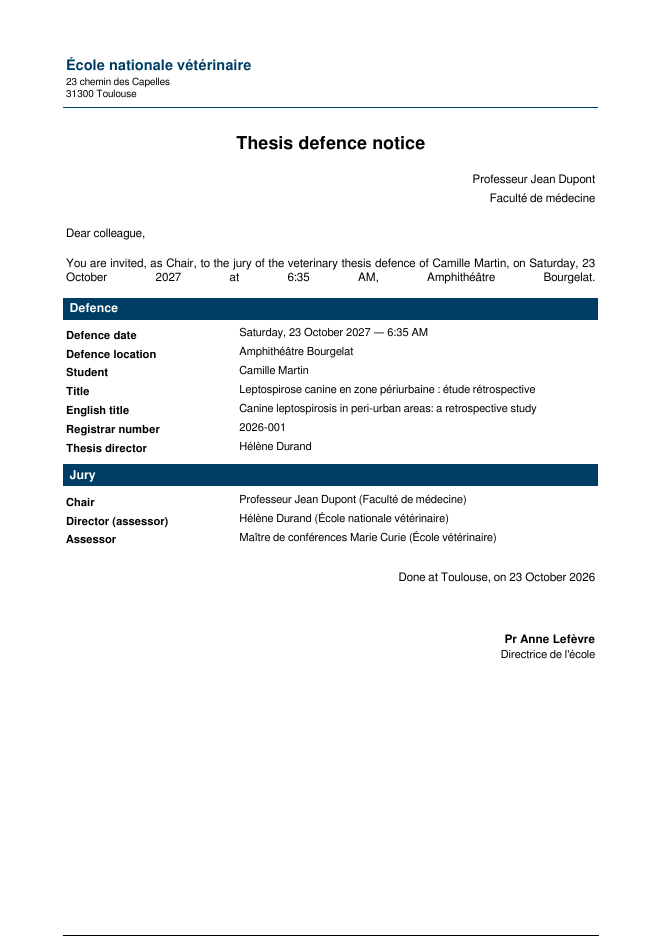
\includegraphics[width=0.46\linewidth]{images/30_convocation}}\hfill
\fcolorbox{cadre}{white}{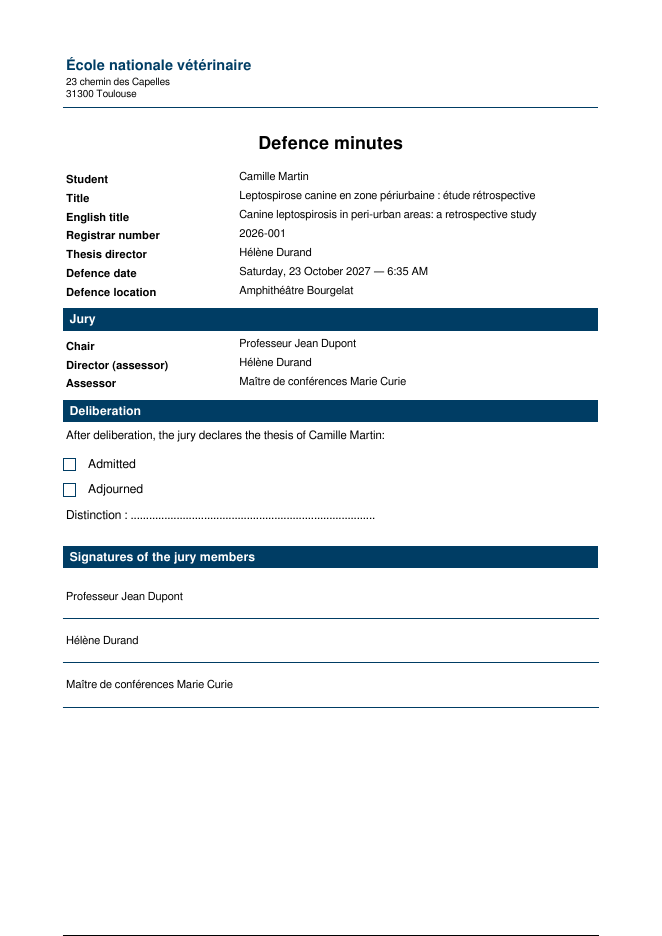
\includegraphics[width=0.46\linewidth]{images/31_proces_verbal}}
\caption{Convocation d'un membre du jury et procès-verbal à signer.}
\end{figure}

\begin{astuce}
Si la date, le lieu ou le jury changent après la génération (via
\bouton{Modifier le dossier}), les documents sont marqués comme à régénérer :
la transmission n'est possible qu'après une nouvelle génération.
\end{astuce}

\subsection{Déposer le procès-verbal (phase 2, étape 6)}

Après la soutenance, \bouton{Déposer le procès-verbal} : PV signé
(obligatoire), résultat (admis, ajourné) et mention éventuelle. Le dépôt clôt le
dossier ; l'étudiant et le directeur sont prévenus.

\subsection{Autres actions}

\begin{description}
  \item[Modifier le dossier] corriger le sujet, changer de directeur, rectifier
        un numéro, reporter la soutenance, modifier le jury, sans changer le
        statut.
  \item[Abandonner / rouvrir] l'abandon, motivé, conserve le dossier tel quel ;
        la réouverture lui rend le statut atteint.
  \item[Créer un dossier] pour un étudiant inscrit qui n'en a pas encore.
\end{description}

% ===========================================================================
\section{Bibliothèque}

\begin{description}
  \item[Phase 1, étape 4] \bouton{Enregistrer le sujet (bibliothèque)} :
        saisir la référence de la notice créée dans le référentiel documentaire.
        Le dossier devient actif ; l'étudiant et son directeur en sont prévenus.
  \item[Phase 2, étape 4] \bouton{Contrôler la conformité du manuscrit} :
        cocher l'attestation de conformité (forme, dépôt légal, normes de
        présentation) et valider, ou renvoyer le dossier à l'étudiant avec le
        motif. L'attestation de conformité est ensuite téléchargeable en PDF
        depuis le dossier.
\end{description}

\capture{13_bibliotheque_conformite}{Contrôle de conformité du manuscrit.}

% ===========================================================================
\section{Courriels et relances}
\label{sec:relances}

\begin{center}
\small
\begin{tabularx}{\linewidth}{@{}l X@{}}
\toprule
\textbf{Courriel} & \textbf{Envoyé} \\
\midrule
Dossier en attente & à l'acteur suivant, à chaque étape franchie \\
Dossier renvoyé & à l'étudiant ou au directeur, avec le motif \\
Sujet enregistré & à l'étudiant et au directeur, à l'ouverture du dossier \\
Convocation & à l'étudiant et aux membres du jury, avec la convocation PDF \\
Transmission à l'université & à l'adresse de l'université, avec l'archive des documents \\
Dossier clôturé & à l'étudiant et au directeur \\
Relance & à l'acteur attendu, après le délai de relance \\
\bottomrule
\end{tabularx}
\end{center}

Chaque texte est personnalisable par la DEVE (\chemin{Courriels}), avec les
variables indiquées sous chaque courriel, par exemple \var{student} ou \var{url}.

\begin{courriel}{Thèse de \{\{student\}\} : \{\{status\}\}}
Bonjour,\\[2pt]
Le dossier de thèse de \{\{student\}\} (\{\{activity\}\}) attend votre action : \{\{status\}\}.\\[2pt]
Sujet : \{\{title\}\}\\[2pt]
Accéder au dossier : \{\{url\}\}
\end{courriel}

Une tâche planifiée quotidienne (7 h 15) relance l'acteur attendu lorsqu'un
dossier attend à la même étape depuis le délai de relance de l'activité
(14 jours par défaut), puis de nouveau à chaque délai écoulé. Les brouillons et
les dossiers actifs ne sont jamais relancés ; un délai de 0 désactive les
relances.

% ===========================================================================
\section{Données personnelles et sauvegarde}

Le module implémente l'API de confidentialité de Moodle : l'étudiant peut
exporter son dossier (sans le rapport du directeur) et en demander
l'effacement ; un membre du personnel supprimé est dissocié des dossiers qu'il a
traités, sans que ceux-ci disparaissent. La sauvegarde et la restauration de
cours recopient le paramétrage et, si les données utilisateur sont incluses,
les dossiers, leur jury, leur historique et leurs fichiers.

\end{document}
